\chapter{Metodologia}
\label{chap:metod}

Para o desenvolvimento deste estudo do Estado da Arte dos robôs antropormóficos foi utilizada a metodologia do método BILI (Bibliographic and Literary Review Method), a qual será explicada nos tópicos seguintes.

\section{Método bili}
\label{sec:bili}

O método BILI (Bibliographic and Literary Review Method) é uma metodologia de pesquisa para o estudo das revisões bibliográficas que visa otimizar a busca e a seleção das referências. Este método é composto por quatro fases e utiliza  ferramentas como o  Rstudio, o Cmaptools e o Mendeley para a seleção, revisão e organização das documentações encontradas. Através desta metodologia é possível encontrar os artigos e autores mais relevantes para a pesquisa.

\begin{figure} [H]	
    \centering
    \caption{Ciclos do método BILI}
    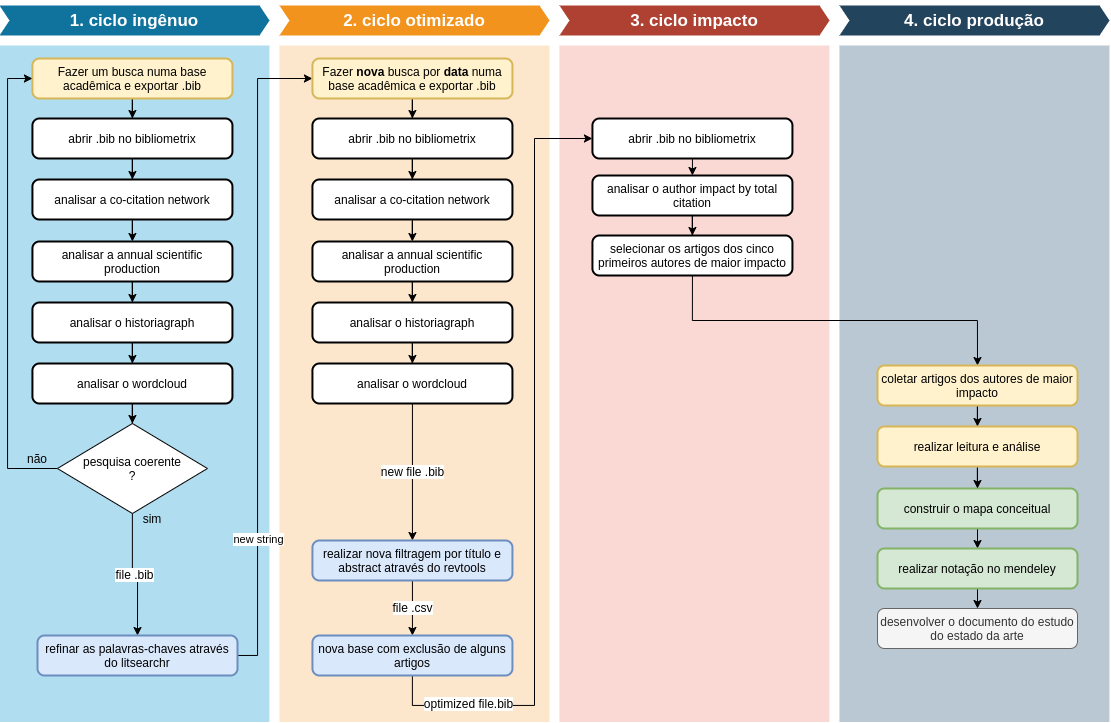
\includegraphics[width=0.6\textwidth]{bili}
    % \caption*{Fonte: Autoria própria.}
    \label{fig:bili}
\end{figure}

\subsection{Fase 1}
\label{sec:fase1}

A primeira fase é denominada de ciclo ingênuo e corresponde a pesquisa inicial feita em uma base acadêmica  de onde foi exportado o arquivo .bib. Através deste arquivo utilizando a ferramenta biblioshiny, fornecida pelo pacote Bibliometrix, foi feita uma análise da rede de co-citação, da produção científica anual e das palavras que aparecem com maior frequência nos artigos. Caso estas informações estejam coerentes com a pesquisa desejada, o pacote litsearchr é utilizado para auxiliar no refinamento da pesquisa através das palavras-chaves. Se o resultado obtido não for satisfatório a busca na base acadêmica deve ser refeita. E, por fim, foi gerada uma nova string que foi utilizada para realizar uma nova busca. 


\subsection{Fase 2}
\label{sec:fase2}

A fase dois é chamada de ciclo otimizado pois, nesta fase foi feita uma nova busca na base acadêmica porém, utilizando as palavras-chaves refinadas. Desta forma, o passo seguinte foi realizar a mesma análise feita no primeiro ciclo e, após está análise foi feita uma filtragem dos artigos utilizando o Revtools. Esta ferramenta permite o pesquisador selecionar os melhores artigos para sua pesquisa através da leitura dos títulos e abstracts. E, então foi exportado um novo arquivo .bib com os dados otimizados para a pesquisa. 

\subsection{Fase 3}
\label{sec:fase3}

Na terceira fase, denominada ciclo impacto, foi feita a análise do impacto do autor utilizando o bibliometrix. E, então foram selecionados os artigos dos cinco primeiros autores de maior impacto.

\subsection{Fase 4}
\label{sec:fase4}

Na última fase, chamada de ciclo produção, é feita a leitura e análise dos artigos selecionados no ciclo anterior e então foi construído um mapa conceitual sobre a pesquisa assim como, todos os artigos selecionados foram armazenados no Mendeley, onde também foram feitas algumas anotações. E, por fim, foi desenvolvida esta documentação com base nestas análises.


% \section{Construção do relatório}
% \label{sec:const}


